\documentclass{article}
\usepackage{bm}
\usepackage{amsmath}
\usepackage{graphicx}
\usepackage{mdwlist}
\usepackage[colorlinks=true]{hyperref}
\usepackage{geometry}
\usepackage{kotex}
\usepackage{adjustbox}
\geometry{margin=1in}
\geometry{headheight=2in}
\geometry{top=2in}
\usepackage{palatino}
%\renewcommand{\rmdefault}{palatino}
\usepackage{fancyhdr}

\newcommand{\red}[1]{{\color{red} #1}}
\newcommand{\blue}[1]{{\color{blue} #1}}
\newcommand{\orange}[1]{{\color{orange} #1}}
\newcommand{\purple}[1]{{\color{purple} #1}}

%\pagestyle{fancy}
\rhead{}
\lhead{}
\chead{%
  {\vbox{%
      \vspace{2mm}
      \large
      Hardware System Design 4190.309A\hfill
\\
      Seoul National University
      \\[4mm]
      \textbf{Final Project. V0 \& Optimization}\\
      \textbf{Jiwon Lee, Sangjun Son}
    }
  }
}

%%%%%%%%%%%%%%%%%%%%%%%
\usepackage{xcolor}
\usepackage{listings}
\definecolor{vgreen}{RGB}{104,180,104}
\definecolor{vblue}{RGB}{49,49,255}
\definecolor{vorange}{RGB}{255,143,102}

\lstdefinestyle{verilog-style}
{
    language=Verilog,
    basicstyle=\scriptsize\ttfamily,
    keywordstyle=\color{vblue},
    identifierstyle=\color{black},
    commentstyle=\color{vgreen},
    numbers=left,
    numberstyle=\tiny\color{black},
    numbersep=10pt,
    tabsize=8,
    moredelim=*[s][\colorIndex]{[}{]},
    literate=*{:}{:}1
}
\lstdefinestyle{c-style}
{
    language=C,
    basicstyle=\scriptsize\ttfamily,
    keywordstyle=\color{vblue},
    identifierstyle=\color{black},
    commentstyle=\color{vgreen},
    numbers=left,
    numberstyle=\tiny\color{black},
    numbersep=10pt,
    tabsize=8,
    moredelim=*[s][\colorIndex]{[}{]},
    literate=*{:}{:}1
}
\lstdefinestyle{python-style}
{
    language=Python,
    basicstyle=\scriptsize\ttfamily,
    keywordstyle=\color{vblue},
    identifierstyle=\color{black},
    commentstyle=\color{vgreen},
    numbers=left,
    numberstyle=\tiny\color{black},
    numbersep=10pt,
    tabsize=8,
    moredelim=*[s][\colorIndex]{[}{]},
    literate=*{:}{:}1
}

\makeatletter
\newcommand*\@lbracket{[}
\newcommand*\@rbracket{]}
\newcommand*\@colon{:}
\newcommand*\colorIndex{%
    \edef\@temp{\the\lst@token}%
    \ifx\@temp\@lbracket \color{black}%
    \else\ifx\@temp\@rbracket \color{black}%
    \else\ifx\@temp\@colon \color{black}%
    \else \color{vorange}%
    \fi\fi\fi
}
\makeatother

\usepackage{trace}
%%%%%%%%%%%%%%%%%%%%%%%

\usepackage{paralist}

\usepackage{todonotes}
\setlength{\marginparwidth}{2.15cm}

\usepackage{tikz}
\usetikzlibrary{positioning,shapes,backgrounds}

\begin{document}

\pagestyle{fancy}

\section*{Goal}

\begin{itemize*}
\item Term Project V0
\begin{itemize*}
\item Implement 8x8 Matrix Matrix multiplication accelerator.
\begin{itemize*}
\item Accuracy on the classification task with CNN should be 100\%.
\item The PE controller should consist of (at most) 8x8 (=64) PEs.
\item The FSM should consist of 5 states: IDLE - LOAD - CALC - HARV - DONE
\item During HARV(harvest) state, the PE controller should write back the computed data to BRAM.
\end{itemize*}
\end{itemize*}
\item Term Project Optimized Version \red{(Optional)}
\begin{itemize*}
\item \textit{DMA} boots data transfer speed between DRAM and BRAM.
\item \textit{Quantization} maps both activation and weights to 8 bit integer.
\item \textit{Zero Skipping} avoids multiplication with zeroes to save computation time.
\end{itemize*}
\end{itemize*}

\section{Implementation}
Final project V0에서는 기존 Lab 6~\cite{lab6}에서 pe\_controller를 구현한 V*V multiplier를 M*M multiplier로 확장한 FPGA accelerator를 구현하는 것을 목표로 한다. 최종적으로 Processing System + BRAM + Connectivity + Custom IP (M*M) 이와 같은 하드웨어 시스템을 만들고 소프트웨어 코드를 이용하여 Convolution lowering on my Custom IP (M*M) on FPGA를 실행하게 된다. \\

\begin{figure}[ht]
	\centering
	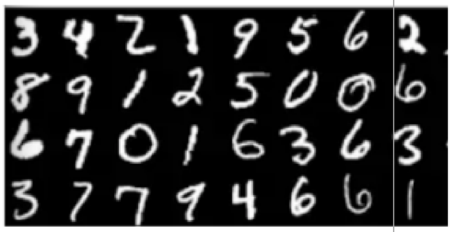
\includegraphics[width=0.6\textwidth]{fig/mnist.png}
\caption{Sample Input Images from MNIST dataset.}
\label{fig1}
\end{figure}

Figure~\ref{fig1}에서 볼 수 있듯이 MNIST 데이터 셋의 입력은 28 x 28 크기의 숫자 이미지이며 이를 벡터화 하여 여러 Layer를 거쳐 마지막에 output layer에 10개의 숫자 중 나타날 확률을 학습하게 된다. 행렬과 벡터 곱셈이 매우 크므로 공간이나 시간적 복잡도를 최적화하기 위해서는 Tiling method를 사용하였으며 이 방법을 CNN 모델의 행렬 곱셈에서도 사용하게 된다. 행렬과 벡터 또는 행렬과 행렬을 일정한 크기로 나누어 가속기를 통해 쓰레드를 나누어 빠른 연산 속도를 가능하게 한다~\cite{lab9}. \\

\newpage
결론적으로 프로젝트에서 구현해야 하는 사항은 다음과 같다.
\begin{enumerate}
    \item \textit{Verilog Matrix-Matrix Multiplication Module}\\
    Lab 6의 PE controller를 변형시켜 Vector-Vector Multiplication Module을 만들고 같은 방식으로 Matrix-Vector Multiplication Module을 구현할 수 있다.
    \item \textit{C Matrix-Matrix Multiplication \& MNIST Classification Module}\\
    위에서 구현한 FPGA 가속기를 사용하거나 CPU를 이용하여 연산할 지에 따라 MNIST Classification을 수행하는 SW 차원의 모듈을 구현해야 한다. 
    \item \textit{Simulation \& Board Implementation} \\
    만들어진 Verilog 모듈을 보드에 올려서 실행하기 전에 Testbench를 만들어 시뮬레이션을 하고 모듈 간의 연결 작업을 시켜준다.
\end{enumerate}

\begin{figure}[htb!]
	\centering
	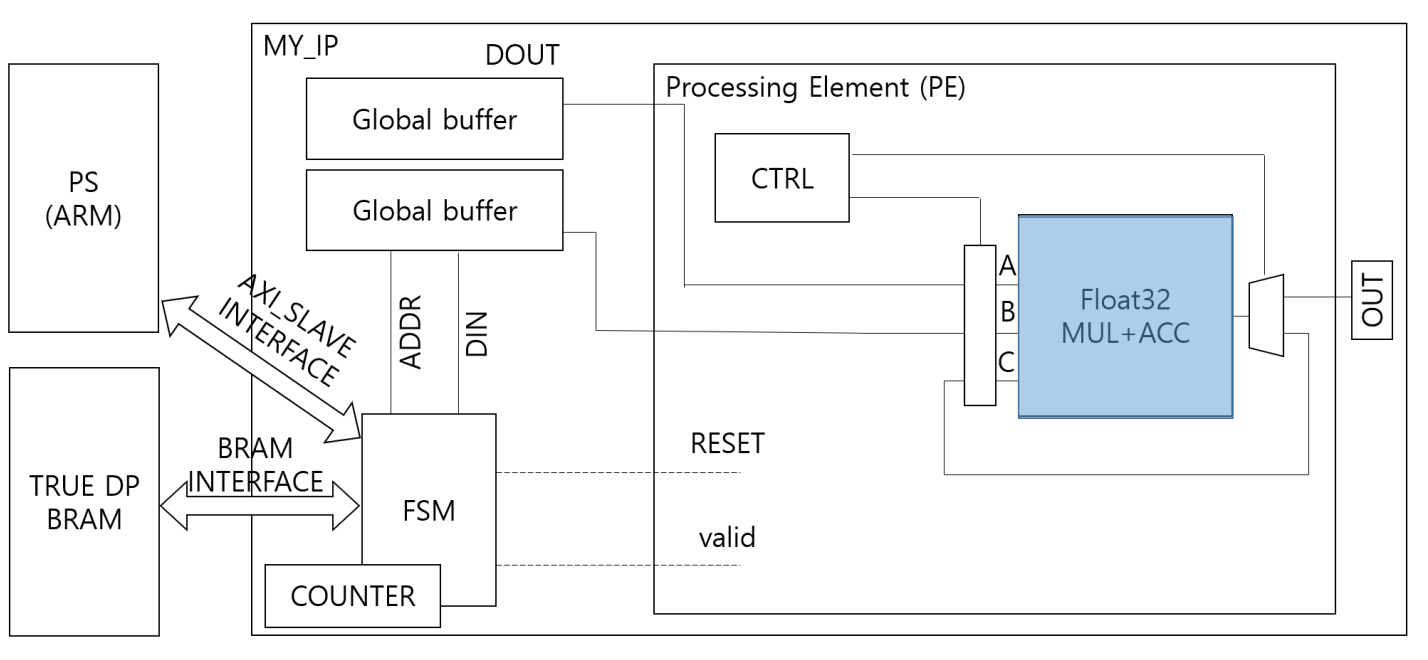
\includegraphics[width=1\textwidth]{fig/overview.png}
\caption{System Overview of the Final Project.}
\label{fig2}
\end{figure}

\subsection{Verilog Matrix-Matrix Multiplication Module}
\label{sec:mm}
Matrix-Matrix Multiplication을 구현하기 위해서는 Lab 6에서 만들었던 Floating point MAC가 포함된 PE controller 모듈이 필요하다. Vivado 프로젝트에서 import를 하여 \texttt{My\_PE}를 추가해주었으며 해당 코드는 Lab 6 보고서 및 프로젝트 제출물에 함께 첨부하였다. \\

PE가 구현이 되었다면 Figure~\ref{fig2}에 있는 \texttt{MY\_IP}에 있는 PE를 다루는 모듈을 구현하면 된다. 행렬 곱셈 기능을 하므로 이름에 맞게 \texttt{mm\_multiplier}라고 하였다. 모듈의 명세에는 그 안에서 사용되는 변수들에 대한 환경 변수인 Buffer의 크기 (\texttt{L\_RAM\_SIZE})와 연산에 사용되는 자료형의 크기 (\texttt{BITWIDTH})가 있다. 환경 변수에 맞게 global buffer, out, counter, address들의 size를 parameter를 사용해 설정하였다. \\

\newpage
아래에 구현한 모듈에 대해 코드와 함께 설명이 진행된다.

\subsection*{Module \texttt{mm\_multiplier.v}}
\begin{lstlisting}[style={verilog-style}]
`timescale 1ns / 1ps

module mm_multiplier #(
    parameter L_RAM_SIZE = 6,
    parameter BITWIDTH = 32
)(
    input start,
    input reset,
    input clk,
    output [2*L_RAM_SIZE:0] rdaddr,
    output [2*L_RAM_SIZE:0] wraddr,
    input [BITWIDTH-1:0] rddata,
    output [BITWIDTH-1:0] wrdata,
    output we,
    output done
);
    localparam DONE_LATENCY = 5;
    localparam S_IDLE = 3'd0, S_LOAD = 3'd1, S_CALC = 3'd2, S_HARV = 3'd3, S_DONE = 3'd4;
    localparam MATRIX_SIZE = 2**(L_RAM_SIZE*2);
    localparam VECTOR_SIZE = 2**(L_RAM_SIZE);
    
    reg [2:0] present_state, next_state;
    reg [2*L_RAM_SIZE:0] cnt_load, cnt_harv;
    reg [L_RAM_SIZE:0] cnt_calc;
    reg [2:0] cnt_done;
    reg rst_cnt_load, rst_cnt_calc, rst_cnt_harv, rst_cnt_done;
    
    reg [BITWIDTH-1:0] gb1[0:MATRIX_SIZE-1];
    reg [BITWIDTH-1:0] gb2[0:MATRIX_SIZE-1];
    reg [BITWIDTH-1:0] data[0:MATRIX_SIZE-1];
    
    reg [BITWIDTH-1:0] ain[0:VECTOR_SIZE-1];
    reg [BITWIDTH-1:0] bin[0:VECTOR_SIZE-1];
    reg valid = 0;
    
    wire [BITWIDTH-1:0]  out[0:MATRIX_SIZE-1];
    wire [BITWIDTH-1:0] dout[0:MATRIX_SIZE-1];
    wire dvalid;
    
    always @(posedge clk or posedge reset)
        if (reset) present_state <= S_IDLE; else present_state <= next_state;
    always @(posedge clk or posedge rst_cnt_load) 
        if (rst_cnt_load) cnt_load <= 0; else cnt_load <= cnt_load + 1;
    always @(posedge clk or posedge rst_cnt_calc) 
        if (rst_cnt_calc) cnt_calc <= 0;
    always @(posedge clk or posedge rst_cnt_harv) 
        if (rst_cnt_harv) cnt_harv <= 0; else cnt_harv <= cnt_harv + 1;
    always @(posedge clk or posedge rst_cnt_done) 
        if (rst_cnt_done) cnt_done <= 0; else cnt_done <= cnt_done + 1;
    
    always @(*)
        case (present_state)
            S_IDLE: if (start)                          next_state = S_LOAD; else next_state = present_state;
            S_LOAD: if (cnt_load == MATRIX_SIZE*2-1)    next_state = S_CALC; else next_state = present_state;
            S_CALC: if (cnt_calc == VECTOR_SIZE)        next_state = S_HARV; else next_state = present_state;
            S_HARV: if (cnt_harv == MATRIX_SIZE-1)      next_state = S_DONE; else next_state = present_state;
            S_DONE: if (cnt_done == DONE_LATENCY-1)     next_state = S_IDLE; else next_state = present_state;
        endcase
    
    always @(*)
        case (present_state)
            S_LOAD: rst_cnt_load <= 0;
            S_CALC: rst_cnt_calc <= 0;
            S_HARV: rst_cnt_harv <= 0;
            S_DONE: rst_cnt_done <= 0;
            default: begin
                rst_cnt_load <= 1; 
                rst_cnt_calc <= 1;
                rst_cnt_harv <= 1;
                rst_cnt_done <= 1;
            end
        endcase
        
    always @(rddata or present_state)
        if (present_state == S_LOAD) 
            if (cnt_load < MATRIX_SIZE) gb1[cnt_load]             = rddata; 
            else                        gb2[cnt_load-MATRIX_SIZE] = rddata;
        
    integer j;
    always @(present_state)
        if (present_state == S_HARV)
            for (j = 0; j < MATRIX_SIZE; j = j+1)
                data[j] <= out[j];
    
    always @(dvalid or present_state)
        if (present_state == S_CALC)
            if (dvalid) begin
                cnt_calc <= cnt_calc + 1;
                valid <= 0;
            end
            else begin
                for (j = 0; j < VECTOR_SIZE; j = j+1) begin
                    ain[j] <= gb1[j*VECTOR_SIZE + cnt_calc];
                    bin[j] <= gb2[cnt_calc*VECTOR_SIZE + j];
                end
                valid <= 1;
            end
    
    assign rdaddr = (present_state == S_LOAD) ? cnt_load : 0;
    assign wrdata = (present_state == S_HARV) ? data[cnt_harv] : 0;
    assign wraddr = (present_state == S_HARV) ? cnt_harv : 0;
    assign we     = (present_state == S_HARV);
    assign done   = (present_state == S_DONE);
    
    genvar i;
    generate for (i = 0; i < MATRIX_SIZE; i = i+1) begin: MATRIX
        my_pe #(L_RAM_SIZE, BITWIDTH) MY_PE(
            .aclk(clk),
            .aresetn(~reset),
            .ain(ain[i/VECTOR_SIZE]),
            .bin(bin[i%VECTOR_SIZE]),
            .valid(valid),
            .dvalid(dvalid),
            .dout(dout[i])
        );
        assign out[i] = present_state == S_HARV ? dout[i] : 0;
    end endgenerate
endmodule
\end{lstlisting}
mm\_multiplier는 PE Controller에서 확장된 구조를 가지고, 따라서 동일한 FSM의 논리를 통해 구현하였다. PE Controller에서 확장된 점은, Matrix-Matrix multiply를 위한 Matrix를 Global buffer에 저장한 뒤, PE에 전달, 이후 연산을 진행한다는 것이다.\\

mm\_multiplier는 IDLE, LOAD, CALC, HARV, DONE의 5가지 state를 가진다. IDLE은 대기 상태를 의미하며, 이 때 \texttt{start} 신호가 입력되면 LOAD state로 전이된다. 이 상태에서는 \texttt{rdaddr} 주소를 Testbench에 전달하여 \texttt{rddata} 값을 하나씩 입력받아 Global buffer에 저장한다.

\newpage
\begin{figure}[ht]
	\centering
	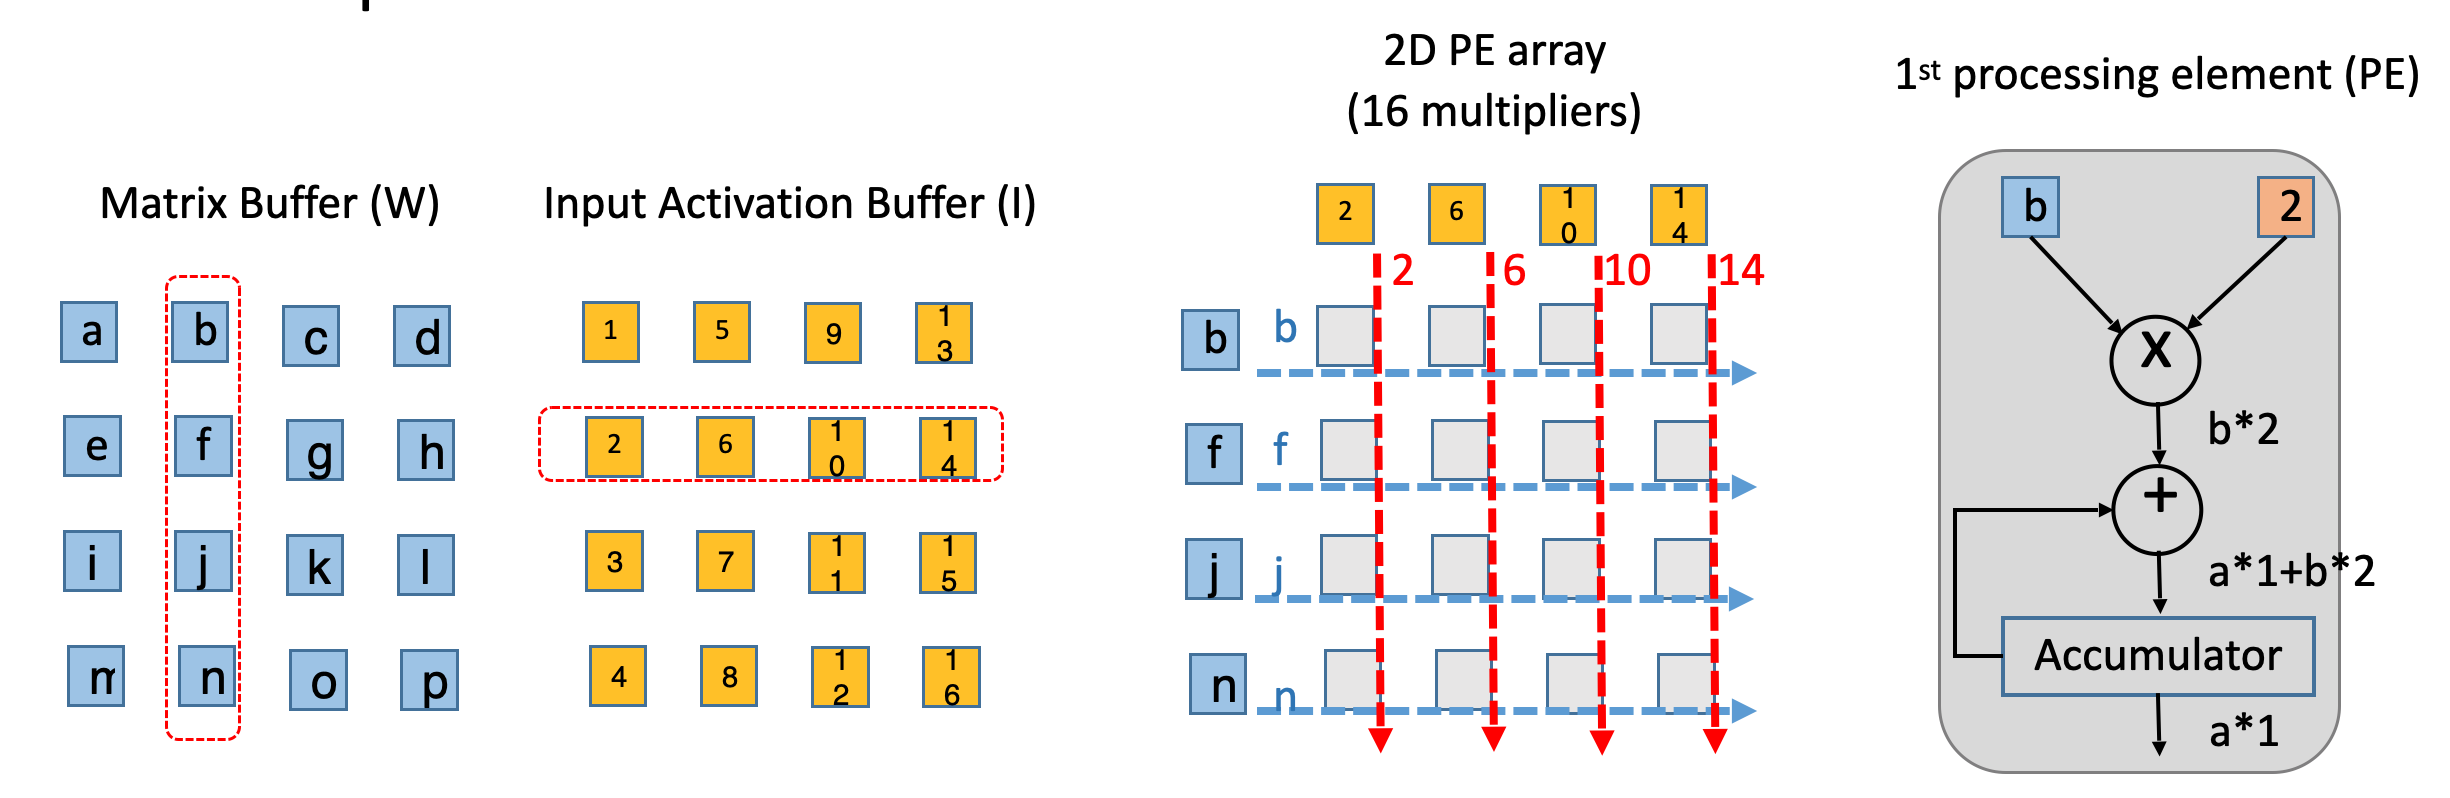
\includegraphics[width=0.8\textwidth]{fig/broadcast_mm.png}
\caption{Broadcast \& PE computation process}
\label{fig3}
\end{figure}
모든 LOAD 과정이 끝나면, Figure~\ref{fig3}에서의 방법과 같은 방식으로, CALC 단계에서 FP IP catalog를 수행하게 된다. Global buffer에 저장된 VECTOR\_SIZE(=64)크기의 열벡터와 행벡터를 추출하여 Multiply-Accumulator를 이용해 내적 값을 구하게 된다. Multiply-Accumulator연산이 모두 끝난 후, \texttt{cnt\_calc}값은 1증가하고, 다음 사이클을 진행한다. 모든 MM연산을 마치면, state는 HARV로 넘어가고, 최종 결과 Matrix와 wrdata를 통해 결과값을 저장한다. 이후, state는 DONE으로 넘어가게 되고 5(Latency)사이클 동안 \texttt{done} signal을 출력한다. 이후에는 다시 state를 IDLE 상태로 돌려 놓고 \texttt{start} 신호를 기다린다.\\
\begin{itemize*}
\item 상기된 코드 중 7-38 라인은 MM multiplier의 변수 선언에 관한 내용이다.
\begin{itemize*}
\item \texttt{parameter}에 포함된 (1) \texttt{L\_RAM\_SIZE}는 입력되는 Matrix의 크기를 표현하는 상수이고, (2) \texttt{BITWIDTH}는 연산을 하기 위한 실수 자료형의 크기를 나타낸다.
\item FSM과 관련된 변수는 현재 상태와 앞으로 업데이트해야하는 상태 변수 \texttt{present\_state}와 \texttt{next\_state}가 있고 그 외에 Counter가 있다. 상태를 나타내는 상수는 총 5가지로 $0 \sim 4$의 값을 \texttt{S\_IDLE}, \texttt{S\_LOAD}, \texttt{S\_CALC}, \texttt{S\_HARV}와 \texttt{S\_DONE}에 해당하도록 설정하였다.
\item 내장 모듈인 MY\_PE의 입출력 변수 \texttt{ain}, \texttt{bin}, \texttt{valid}, \texttt{dout}, \texttt{dvalid}를 함께 선언하고 지정시켜주어야 한다.
\end{itemize*}

\item 40-49 라인과 51-58 라인은 강의시간에 배운 FSM의 format을
그대로 차용하여 구현하였다. 초기 상태를 \texttt{reset} 신호와 함께 IDLE 상태로 초기화 한다. 현재 상태에서 어떤 조건이 중족되었을 때 다음 상태를 지정해주는 논리를 구현해준다.

\item 60-103라인은 각 상태에 위치했을 때 어떤 Counter를 활성화 시킬지 지정해주는 부분이다. 74-77라인에서는 현재 상태가 LOAD에 이르렀을 때 테스트벤치로 \texttt{rdaddr}을 전달해주고 해당하는 실수형 자료 \texttt{rddata}를 받아와 Global buffer에 저장한다.

\item 105-117라인은 \texttt{generate}문에서 PE 모듈 인스턴스를 생성하여, Matrix-Matrix multiply를 수행한다.
\end{itemize*}

\newpage
\section{Result}
아래의 코드는 mm\_multiplier를 검증하기 위한 testbench코드이다.
\subsection*{Testbench Module \texttt{tb\_mm\_multiplier.v}}
\begin{lstlisting}[style={verilog-style}]
`timescale 1ns / 1ps

module tb_mm_multiplier #(
    parameter L_RAM_SIZE = 3,
    parameter BITWIDTH = 32,
    parameter INFILE = "global_buffer_in.txt",
    parameter OUTFILE = "global_buffer_out.txt"
)();
    localparam MATRIX_SIZE = 2**(L_RAM_SIZE*2);
    localparam VECTOR_SIZE = 2**(L_RAM_SIZE);
    reg [BITWIDTH-1:0] rdgb[0:MATRIX_SIZE*2-1];
    reg [BITWIDTH-1:0] wrgb[0:MATRIX_SIZE-1];
    wire [BITWIDTH-1:0] rddata;
    wire [BITWIDTH-1:0] wrdata;
    wire [2*L_RAM_SIZE:0] rdaddr;
    wire [2*L_RAM_SIZE:0] wraddr;
    wire done, we;
    
    reg start, clk, reset;
//    integer i;
//    initial begin
//        for(i = 0; i < MATRIX_SIZE; i = i+1) begin
//            rdgb[i]               = $urandom_range(2**30, 2**30+2**24);
//            rdgb[MATRIX_SIZE + i] = $urandom_range(2**30, 2**30+2**24);
//        end
//        $writememh(INFILE, rdgb);
//    end
    assign rddata = start ? rdgb[rdaddr] : 0;
    initial begin
        $readmemh(INFILE, rdgb);
        clk <= 0;
        start <= 0; reset <= 1;
        #10 start <= 1; reset <= 0;
    end
    always @(*)
        if (we) wrgb[wraddr] = wrdata;
    always @(posedge done)
        $writememh(OUTFILE, wrgb);
    
    always #1 clk = ~clk;
    mm_multiplier #(L_RAM_SIZE, BITWIDTH) MM_MULTIPLIER(
        .start(start),
        .reset(reset),
        .clk(clk),
        .rdaddr(rdaddr),
        .rddata(rddata),
        .we(we),
        .wraddr(wraddr),
        .wrdata(wrdata),
        .done(done)
    );
endmodule
\end{lstlisting}
\newpage
mm\_multiplier모듈의 parameter값들을 tb\_mm\_multiplier모듈의 4-7라인에서 초기화하고, 9-19라인에서 input 및 output값들을 초기화시킨다. Matrix 2개의 값들은 input.txt에 저장한다. input.txt에 저장된 값을 읽어들여, output.txt로 결과값을 출력시킨다. 아래의 waveform은 testbench를 통해 얻어진 결과값이다.

\begin{figure}[htb!]
	\centering
	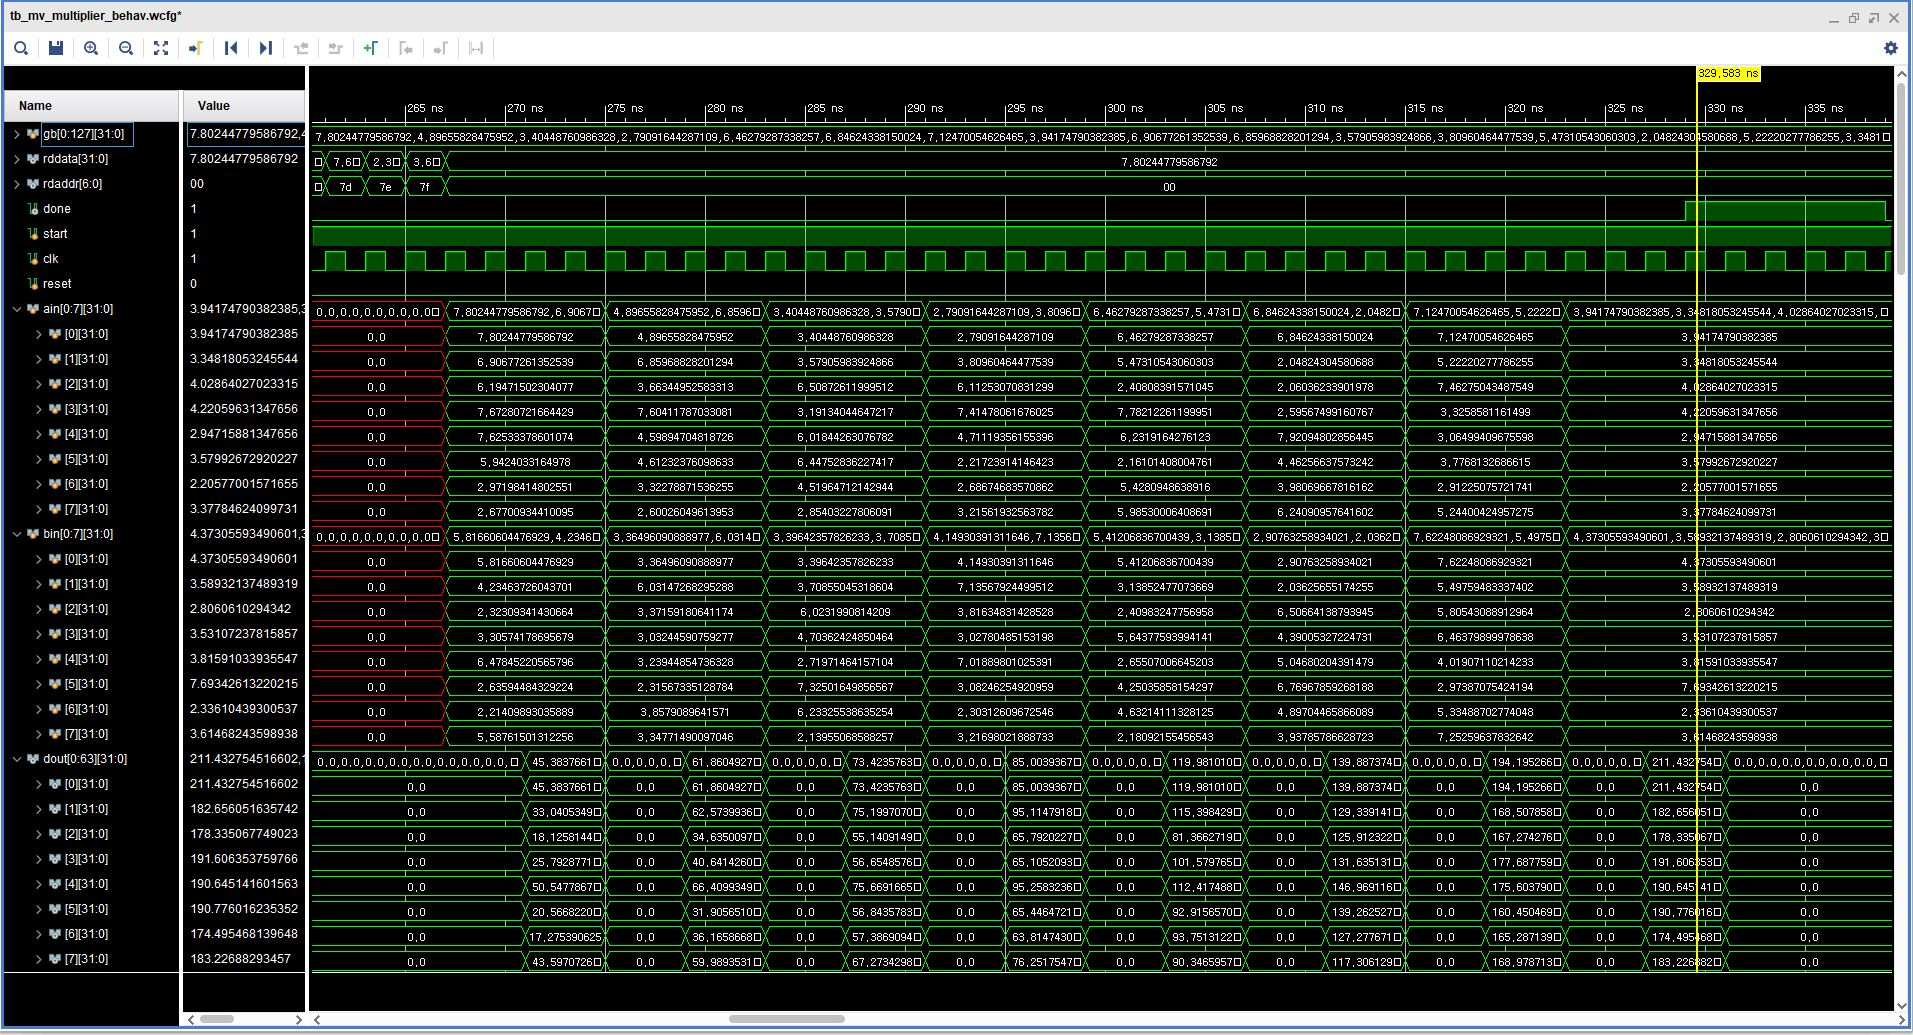
\includegraphics[width=0.9\textwidth]{fig/mm1.jpg}
\caption{Broadcast \& PE computation process}
\label{fig4}
\end{figure}
\begin{figure}[htb!]
	\centering
	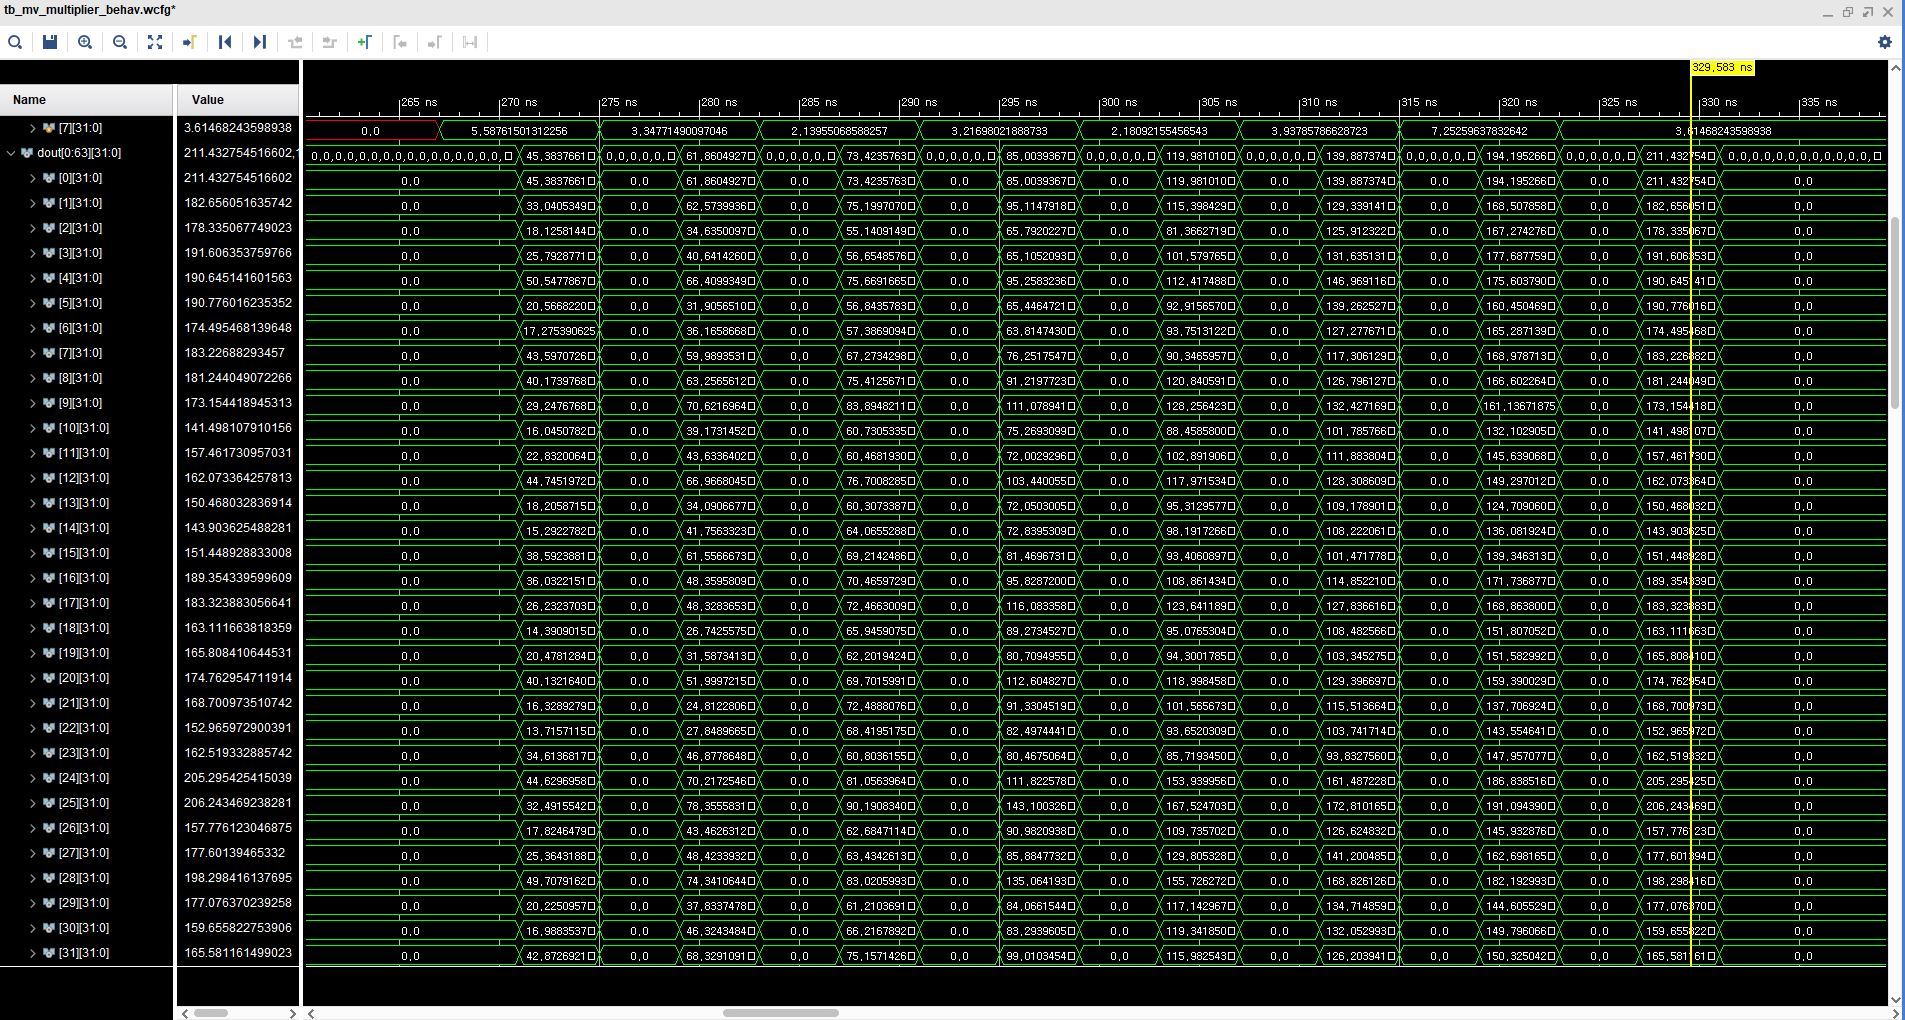
\includegraphics[width=0.9\textwidth]{fig/mm2.jpg}
\caption{Broadcast \& PE computation process}
\label{fig5}
\end{figure}
\begin{figure}[htb!]
	\centering
	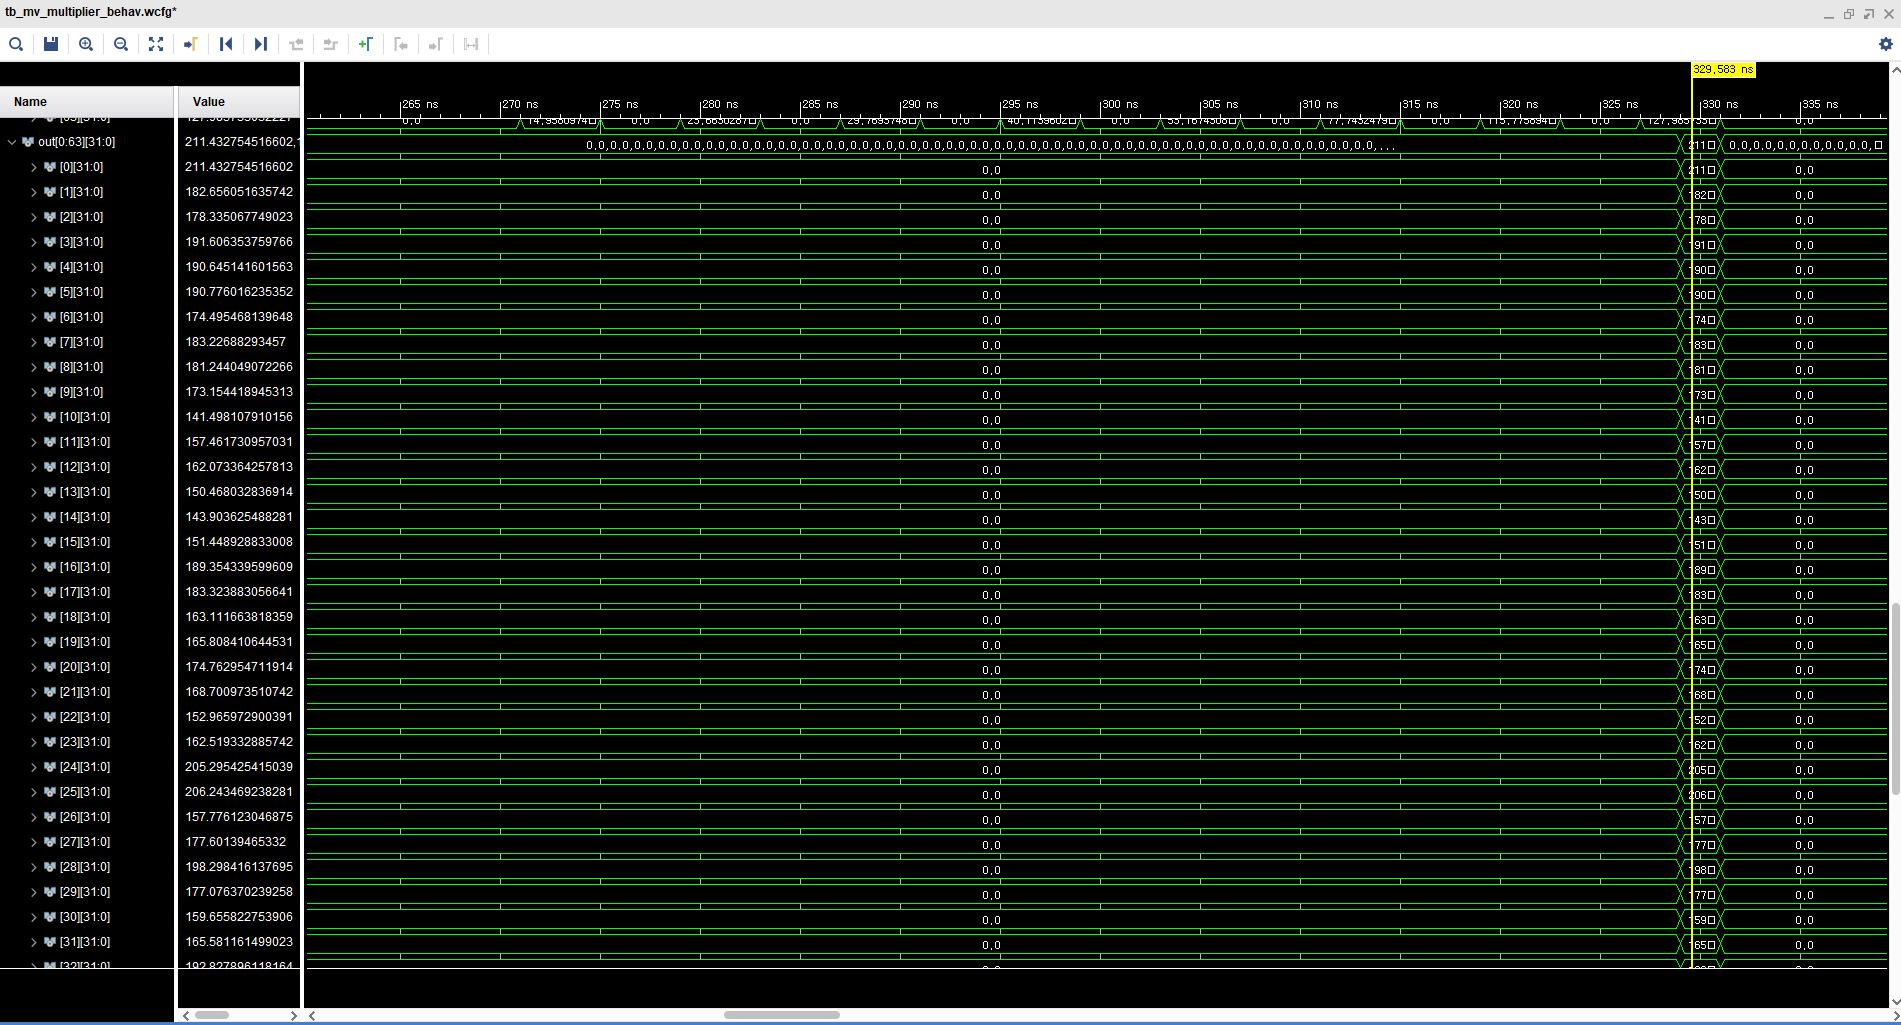
\includegraphics[width=0.9\textwidth]{fig/mm3.jpg}
\caption{Broadcast \& PE computation process}
\label{fig6}
\end{figure}

ain, bin은 PE모듈의 input이고, PE는 내적을 수행하기 때문에, \texttt{ain}은 Matrix-Matrix multiply에서 첫 번째 matrix그대로 들어가고, \texttt{bin}은 두 번째 Matrix의 전치행렬이다. 이를 통해 Figure~\ref{fig3}의 과정이 잘 구현되었다는 것을 알 수 있다.

\subsection*{Testbench Data \texttt{global\_buffer\_mm.txt}}
아래의 표는 테스트벤치에서 생성된 실수 행렬을 저장한 입력 파일에서 행렬 A와 B를 읽어와 모듈 \texttt{mm\_mul}을 통해 연산한 행렬 C를 연산한 결과이다. 표의 상단 부분은 16진수 형태의 single precision floating point 자료형이고 하단부는 Python hex-to-float decoder를 통해 실수 형태로 변환한 결과이다. 행렬 곱셈연산이 제대로 수행됨을 확인할 수 있다.

\newpage
\hfill
\begin{adjustbox}{angle=90}
\resizebox{\textheight}{!}{
\begin{tabular}{|c|rrrrrrrr|c|rrrrrrrr|}
\hline
A & \multicolumn{1}{c}{0} & \multicolumn{1}{c}{1} & \multicolumn{1}{c}{2} & \multicolumn{1}{c}{3} & \multicolumn{1}{c}{4} & \multicolumn{1}{c}{5} & \multicolumn{1}{c}{6} & \multicolumn{1}{c|}{7} & B & \multicolumn{1}{c}{0} & \multicolumn{1}{c}{1} & \multicolumn{1}{c}{2} & \multicolumn{1}{c}{3} & \multicolumn{1}{c}{4} & \multicolumn{1}{c}{5} & \multicolumn{1}{c}{6} & \multicolumn{1}{c|}{7} \\ \hline
0 & 40f9ada7 & 409cb09b & 4059e320 & 40329e60 & 40cecf33 & 40db146d & 40e3fd8c & 407c4599 & 0 & 40ba21a3 & 40878226 & 4014ad90 & 40539146 & 40cf4f7b & 4028b352 & 400db3cc & 40b2cdbe \\
1 & 40dd0448 & 40db8291 & 40650f51 & 4073d090 & 40af23ae & 4003166a & 40a71c49 & 40564897 & 1 & 40575b85 & 40c101d3 & 4057c829 & 40421398 & 404f5320 & 401433fe & 4076e7fb & 405640f6 \\
2 & 40c63b1b & 406a75f5 & 40d0477c & 40c399da & 401a1e0c & 4003dcfa & 40eeceda & 4080ea9f & 2 & 40595f01 & 406d58e4 & 40c0be0c & 40968417 & 402e0fce & 40ea6689 & 40c776d4 & 4008ee66 \\
3 & 40f587a3 & 40f354ef & 404c3eec & 40ed45e2 & 40f90726 & 40261f8a & 4054dadc & 40870f20 & 3 & 4084c719 & 40e4577c & 40743f0d & 4041c78e & 40e09ad0 & 40454711 & 4013666b & 404de301 \\
4 & 40f402bc & 40932a93 & 40c09715 & 4096c219 & 40c76bdc & 40fd7868 & 404428dd & 403c9e40 & 4 & 40ad2faa & 4048dd97 & 401a3ab2 & 40b499d0 & 4029ecab & 408802f0 & 40943a80 & 400b9438 \\
5 & 40be282b & 40939828 & 40ce5227 & 400de73f & 400a4e0e & 408ecd58 & 4071b74f & 40651d85 & 5 & 403a16a7 & 40025207 & 40d03668 & 408c7b51 & 40a17f67 & 40d8a135 & 409cb497 & 407c05dd \\
6 & 403e34fd & 4054a892 & 4090a0f3 & 402bf3a9 & 40adb2f4 & 407ec3bc & 403a6251 & 400d2b56 & 6 & 40f3eb5d & 40afec4c & 40b9c617 & 40ced771 & 40809c3b & 403e53e6 & 40aab765 & 40e81545 \\
7 & 402b541f & 40266aab & 4036a877 & 404dccb5 & 40bf8794 & 40c7b588 & 40a7cee2 & 40582ea2 & 7 & 408bf013 & 4065b771 & 40339681 & 4061fd17 & 407437e0 & 40f6308c & 401582bc & 406756f5 \\ \hline
C & \multicolumn{1}{c}{0} & \multicolumn{1}{c}{1} & \multicolumn{1}{c}{2} & \multicolumn{1}{c}{3} & \multicolumn{1}{c}{4} & \multicolumn{1}{c}{5} & \multicolumn{1}{c}{6} & \multicolumn{1}{c|}{7} &  & \multicolumn{1}{c}{} & \multicolumn{1}{c}{} & \multicolumn{1}{c}{} & \multicolumn{1}{c}{} & \multicolumn{1}{c}{} & \multicolumn{1}{c}{} & \multicolumn{1}{c}{} & \multicolumn{1}{c|}{} \\ \hline
0 & 43536ec9 & 4336a7f3 & 433255c7 & 433f9b3a & 433ea528 & 433ec6a9 & 432e7ed7 & 43373a15 &  &  &  &  &  &  &  &  &  \\
1 & 43353e7a & 432d2788 & 430d7f84 & 431d7634 & 432212c8 & 431677d1 & 430fe754 & 431772ed &  &  &  &  &  &  &  &  &  \\
2 & 433d5ab6 & 433752ea & 43231c96 & 4325cef4 & 432ec351 & 4328b373 & 4318f74a & 432284f3 &  &  &  &  &  &  &  &  &  \\
3 & 434d4ba1 & 434e3e54 & 431dc6b0 & 433199f5 & 43464c65 & 4331138d & 431fa7e4 & 432594c7 &  &  &  &  &  &  &  &  &  \\
4 & 4340d3f1 & 4333152d & 433411f4 & 4335e3bb & 4341d207 & 43494175 & 432de216 & 4323b37a &  &  &  &  &  &  &  &  &  \\
5 & 43164c64 & 430e329f & 430ede1e & 430b82f3 & 430fa2e2 & 431e937f & 43089f44 & 430430b0 &  &  &  &  &  &  &  &  &  \\
6 & 42ff8693 & 42eb4228 & 42eb52cf & 42f8091f & 42e7952b & 43049116 & 42ee2c16 & 42cd4d8f &  &  &  &  &  &  &  &  &  \\
7 & 4318a3d3 & 4304ff07 & 430b66c0 & 4312e57d & 430973c0 & 43192a9f & 43074efe & 42fff8b2 &  &  &  &  &  &  &  &  &  \\ \hline
A & \multicolumn{1}{c}{0} & \multicolumn{1}{c}{1} & \multicolumn{1}{c}{2} & \multicolumn{1}{c}{3} & \multicolumn{1}{c}{4} & \multicolumn{1}{c}{5} & \multicolumn{1}{c}{6} & \multicolumn{1}{c|}{7} & B & \multicolumn{1}{c}{0} & \multicolumn{1}{c}{1} & \multicolumn{1}{c}{2} & \multicolumn{1}{c}{3} & \multicolumn{1}{c}{4} & \multicolumn{1}{c}{5} & \multicolumn{1}{c}{6} & \multicolumn{1}{c|}{7} \\ \hline
0 & 7.8024 & 4.8966 & 3.4045 & 2.7909 & 6.4628 & 6.8462 & 7.1247 & 3.9417 & 0 & 5.8166 & 4.2346 & 2.3231 & 3.3057 & 6.4785 & 2.6359 & 2.2141 & 5.5876 \\
1 & 6.9068 & 6.8597 & 3.5791 & 3.8096 & 5.4731 & 2.0482 & 5.2222 & 3.3482 & 1 & 3.3650 & 6.0315 & 3.3716 & 3.0324 & 3.2394 & 2.3157 & 3.8579 & 3.3477 \\
2 & 6.1947 & 3.6634 & 6.5087 & 6.1125 & 2.4081 & 2.0604 & 7.4628 & 4.0286 & 2 & 3.3964 & 3.7086 & 6.0232 & 4.7036 & 2.7197 & 7.3250 & 6.2333 & 2.1396 \\
3 & 7.6728 & 7.6041 & 3.1913 & 7.4148 & 7.7821 & 2.5957 & 3.3259 & 4.2206 & 3 & 4.1493 & 7.1357 & 3.8163 & 3.0278 & 7.0189 & 3.0825 & 2.3031 & 3.2170 \\
4 & 7.6253 & 4.5989 & 6.0184 & 4.7112 & 6.2319 & 7.9209 & 3.0650 & 2.9472 & 4 & 5.4121 & 3.1385 & 2.4098 & 5.6438 & 2.6551 & 4.2504 & 4.6321 & 2.1809 \\
5 & 5.9424 & 4.6123 & 6.4475 & 2.2172 & 2.1610 & 4.4626 & 3.7768 & 3.5799 & 5 & 2.9076 & 2.0363 & 6.5066 & 4.3901 & 5.0468 & 6.7697 & 4.8970 & 3.9379 \\
6 & 2.9720 & 3.3228 & 4.5196 & 2.6867 & 5.4281 & 3.9807 & 2.9123 & 2.2058 & 6 & 7.6225 & 5.4976 & 5.8054 & 6.4638 & 4.0191 & 2.9739 & 5.3349 & 7.2526 \\
7 & 2.6770 & 2.6003 & 2.8540 & 3.2156 & 5.9853 & 6.2409 & 5.2440 & 3.3778 & 7 & 4.3731 & 3.5893 & 2.8061 & 3.5311 & 3.8159 & 7.6934 & 2.3361 & 3.6147 \\ \hline
C & \multicolumn{1}{c}{0} & \multicolumn{1}{c}{1} & \multicolumn{1}{c}{2} & \multicolumn{1}{c}{3} & \multicolumn{1}{c}{4} & \multicolumn{1}{c}{5} & \multicolumn{1}{c}{6} & \multicolumn{1}{c|}{7} &  & \multicolumn{1}{c}{} & \multicolumn{1}{c}{} & \multicolumn{1}{c}{} & \multicolumn{1}{c}{} & \multicolumn{1}{c}{} & \multicolumn{1}{c}{} & \multicolumn{1}{c}{} & \multicolumn{1}{c|}{} \\ \hline
0 & 211.4328 & 182.6561 & 178.3351 & 191.6064 & 190.6451 & 190.7760 & 174.4955 & 183.2269 &  &  &  &  &  &  &  &  &  \\
1 & 181.2440 & 173.1544 & 141.4981 & 157.4617 & 162.0734 & 150.4680 & 143.9036 & 151.4489 &  &  &  &  &  &  &  &  &  \\
2 & 189.3543 & 183.3239 & 163.1117 & 165.8084 & 174.7630 & 168.7010 & 152.9660 & 162.5193 &  &  &  &  &  &  &  &  &  \\
3 & 205.2954 & 206.2435 & 157.7761 & 177.6014 & 198.2984 & 177.0764 & 159.6558 & 165.5812 &  &  &  &  &  &  &  &  &  \\
4 & 192.8279 & 179.0827 & 180.0701 & 181.8896 & 193.8204 & 201.2557 & 173.8831 & 163.7011 &  &  &  &  &  &  &  &  &  \\
5 & 150.2984 & 142.1977 & 142.8676 & 139.5115 & 143.6363 & 158.5762 & 136.6221 & 132.1902 &  &  &  &  &  &  &  &  &  \\
6 & 127.7628 & 117.6292 & 117.6617 & 124.0178 & 115.7913 & 132.5667 & 119.0861 & 102.6515 &  &  &  &  &  &  &  &  &  \\
7 & 152.6399 & 132.9962 & 139.4014 & 146.8964 & 137.4521 & 153.1665 & 135.3086 & 127.9857 &  &  &  &  &  &  &  &  &  \\ \hline
\end{tabular} \newline
}\end{adjustbox}
\hfill
\null

\section{Conclusion}
이번 실습에서 구현한 mm\_multiplier 모듈은 최종 프로젝트를 위한 중간과정이었다. simulation 상에서 동작하는 것을 목표로 진행했기 때문에 보드에서 동작하는 것은 확인하지 않았다. Matrix-Matrix Multiplication를 구현하기 위해서는 PE가 여러 개 필요하였고 이를 위해서는 for generate를 사용하여 코드의 반복을 막을 수 있었고 가독성 또한 높일 수 있었다. \\

프로젝트 V0에서는 Custom IP의 기본이 되는 모듈을 구성한 것이기 때문에, 후에 synthesis, implementation, bitstream generating으로 이어지는 일련의 과정들이 잘 수행되기 위해서는 굉장히 중요한 실습이었을 것이라 생각한다. 


\bibliographystyle{plain}
\bibliography{other}

\end{document}
